
%% Journal of Networking and Network Applications.tex
%% V1.0
%% 2020/01/24
%% see https://iecscience.org/journals/J-NaNA
%% for current contact information.

%%*************************************************************************
%% Legal Notice:
%% This code is offered as-is without any warranty either expressed or
%% implied; without even the implied warranty of MERCHANTABILITY or
%% FITNESS FOR A PARTICULAR PURPOSE! 
%% User assumes all risk.
%% In no event shall the J-NaNA or any contributor to this code be liable for
%% any damages or losses, including, but not limited to, incidental,
%% consequential, or any other damages, resulting from the use or misuse
%% of any information contained here.
%%
%% All comments are the opinions of their respective authors and are not
%% necessarily endorsed by the J-NaNA.
%%*************************************************************************


\documentclass[journal,transmag]{J-NaNA}
\hyphenation{Machine Learning with Graphs}


\usepackage{graphicx} % Include the package

\begin{document}

\title{Prediction of Drug-Induced Side Effects Through A Graph Comprehensive Approach Using BioSNAP and Mambo}



% author names and affiliations
% transmag papers use the long conference author name format.

\author{\NaNAauthorblockN{Nikhil Thota\NaNAauthorrefmark{1},
		Hema Sai Venkata Dumpala\NaNAauthorrefmark{2},
		Saba Shafiei Tehrani\NaNAauthorrefmark{3}, and
		Somna Satoor\NaNAauthorrefmark{4}}
	\NaNAauthorblockA{\NaNAauthorrefmark{1}Department of Applied Data Science, San Jose State University, San Jose, California, US}}



% The paper headers
\markboth{DATA 245: Machine Learning, December 2023}%
{Shell \MakeLowercase{\textit{Nikhil et al.}}: Project Report by Team 6}


\NaNAtitleabstractindextext{
\begin{abstract}
In addressing the complexities of polypharmacy and the associated risks of adverse drug interactions (ADIs), this study leverages the BioSNAP datasets, with a particular focus on the DrugBank dataset. Utilizing Mambo, A real-time data extraction pipeline from DrugBank is re-developed, enabling the cleaning and processing of data for predictive modeling. A key component of this study was the application of a Random Forest algorithm to predict drug half-lives, providing foundational insights into handling and interpreting pharmaceutical data. The research further explores the chse-decagon dataset of BioSNAP, forming bipartite graphs to examine drug-side effect correlations. Due to the complexity of the side-effect graph, the focus shifted to drug nodes. Node2Vec was used for feature extraction, yielding 64-dimensional vectors per node. The processed data were then subjected to stratified splitting, scaling, and SMOTE to address class imbalance. Clustering algorithms, such as K-Nearest Neighbours and HDBScan, were evaluated, with K-means and HDBSCAN ultimately being employed for analyzing drug similarities based on shared side effects. The project culminates in converting the chchse-decagon dataset into a binary classification framework to manage the multifaceted nature of DDI prediction. Utilizing a Graph Neural Network algorithm, the model achieved an 88.9\% accuracy in testing. The developed models, encapsulated as .pkl files, are integrated into a Gradio interface, facilitating real-time classification testing and demonstrating potential applications in healthcare informatics.
\end{abstract}

% Note that keywords are not normally used for peerreview papers.
\begin{NaNAkeywords}
Bi-partite graphs, Node2Vec, Graph Data Modeling, K-Nearest Neighbors, HDBSCAN, Graph Neural Networks, Polypharmacy, Drug-Drug Interactions (DDI) , Adverse drug reactions (ADR)
\end{NaNAkeywords}}



% make the title area
\maketitle


% To allow for easy dual compilation without having to reenter the
% abstract/keywords data, the \NaNAtitleabstractindextext text will
% not be used in maketitle, but will appear (i.e., to be "transported")
% here as \NaNAdisplaynontitleabstractindextext when the compsoc 
% or transmag modes are not selected <OR> if conference mode is selected 
% - because all conference papers position the abstract like regular
% papers do.
\NaNAdisplaynontitleabstractindextext

\NaNApeerreviewmaketitle



\section{Introduction}

\NaNAPARstart{T}{he} practice of polypharmacy, involving the concurrent use of multiple medications by a patient, poses significant risks in healthcare, particularly due to adverse drug reactions (ADRs) and drug-drug interactions (DDIs). These risks are quantifiably significant: ADRs account for about 106,000 deaths annually and represent 6.7\% of hospital admissions, while serious ADRs number over 2,216,000 cases each year. These statistics underscore the urgent need for more effective tools to predict and manage ADRs and DDIs in polypharmacy. This project will segment the drugs based on the side-effects associated against each drug, by studying the graph structure of the components. The drugs clusters created are used to identify the similar drug families causing side-effects. A classifier is also employed to classify whether that particular drug-drug reaction causes a side-effect or not. For the purpose of this project, real time data pipeline implementation to develop Mambo is also illustrated along with Half-life prediction of the drugs. The Classification models for binary classification are evaluated using performance metrics and classification report, Gradio will be used to check the results of classification of drugs interactions.
\subsection{Problem Statement}
Accurate prediction of potential ADRs and DDIs in multi-drug regimens is a complex challenge that directly impacts patient safety. The consequences of these interactions can range from reduced efficacy of treatments to severe, life-threatening side effects. This issue is becoming increasingly critical with an aging global population and a rise in medication usage. The existing solutions for this problem statement is to use Subject matter expertise from various researchers or professionals, this project can be a first step to easily understand the drug-drug interactions and their consequences, and can be easily accessible by common people. 

\subsection{Project Background}
This paper makes use of DrugBank datasets, and BioSNAP datasets to further understand the drug similarities, and side-effect associations based on their Network structure. This project is a baby step towards understanding the drug drug interactions (DDI) causing side-effects, and the side-effects caused by various drugs. The existing work is pretty complex, and requires a lot of domain knowledge to proceed with the current trends, so this project can be defined as the first step towards 'Understanding the drug-drug interactions to common people'. To meet that goal, a clustering algorithm is deployed to group similar drugs based on the number of side-effects they are associated with, and a classification model is also deployed to understand whether a particular DDI causes a side-effect or not. Inital exploration of Mambo is also done by developing a real time data pipeline with the Drugbank database to understand the Half-life prediction of the Drugs. Overall, the project aims to throw more light and highlight the importance of Adverse Drug Reactions, which are caused by various Drug drug interactions.


\section{Related Work}
Recent advances in data analytics and machine learning, particularly in the area of graph theory and network analysis such as the study employed by Ke Han [1] briefly explains various methods of extracting features for Drug-drug interactions. Building on these advancements, while employing comprehensive pharmaceutical datasets, such as BioSNAP, Drugbank, and the exploration of graph-related properties within these datasets. Machine learning models, particularly those leveraging the intricate network of drug interactions and side effects represented in these datasets, have the potential to identify complex drug interactions that are not apparent through conventional pharmacological research methods. Some of these advancements are discussed in the works of Aditya Grover [2], where the authors briefly explain the latest feature extraction techniques that are current industry standards for extracting features for Network datasets. Sunjoo Bang [3] explains how Attention networks can be adapted to Graph use-cases by studying the side-effects prediction with enhanced interpretability based on graph feature attention network. Marinka Zitnik [4], a research team member of the BioSNAP research team from Standford, along with her team published a study on using GNN for side-effect prediction using the BioSNAP datasets. NICHOLAS P. TATONETTI [5] study showcases how comprehensive analysis of observational clinical data, despite its inherent limitations, can significantly enhance the prediction and understanding of adverse drug effects and interactions. This approach marks a substantial advancement in pharmacogenomics, aiming to protect future patients from serious drug-related consequences.
\\
\section{Proposed Method}
In this study, Mambo is a graph network construction tool for BioMedical data to facilitate the extraction of batch and real-time data from the DrugBank and BioSNAP dataset through various techniques. Here, predicting the half-life values for various drugs. This capability is vital for ensuring that our predictive models are built upon the most current and comprehensive drug information available, which includes data on drug properties, interactions, and reported side effects. The primary focus, however is on analyzing and predicting adverse drug reactions (ADRs) and drug-drug interactions (DDIs) within the realm of polypharmacy, using the BioSNAP datasets. The approach involves categorizing drugs into distinct families or groups based on associated side effects. By understanding these relationships, the study aims to discern patterns that could indicate potential risks in drug combinations, and predict whether the DDI causes an adverse drug reaction or not.  
\\
As described in the previous paragraph, these are essentially two different components of this project. So the methodology, and process followed would be different. For Mambo, the focus is on integrating with BioSNAP dataset on batch data and DrugBank Data on real-time basis, apply initial data cleaning, and exploration, feature engineering and then predict the half-life values for various drugs, this architecture is shown in below Figure 1, where the entire architecture is detailed on an overview level.
\\
Basically, In  a graph, There are nodes and edges. For example, Node means an entity or a drug or a disease in the Drug Bank dataset. Grouping of similar nodes is called a mode in the same way For Example Disease-Disease, Drug-Drug etc.,Linking two nodes are called edges or link types or relationships For example, Disease-Drugs. Finally, Linking the different modes with a link type is the basis for Multi-Modal representation. This multi modal network graph representation is constructed by the Mambo tool which is built by SNAP group in Stanford. As it is built by the SNAP group which can be imported by the SNAP package library. But, Internally SNAP library works on Python 2.7 and the present version and most of the people use python 3.x version and also the SNAP library initially built on top C++ programming language.
\\
\begin{figure}[htbp]
\centering
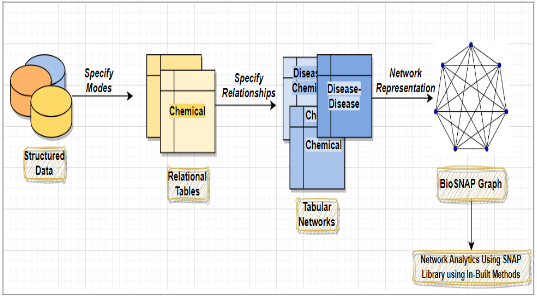
\includegraphics[width=\linewidth]{mambo_arch.PNG} 
\caption{Architecture for Mambo Data Exploration and Prediction}
\label{fig:mambo_architecture} % Label for referencing the image within your text
\end{figure}

\\
Once after the modes and relationships are specified. A graph can be represented to show the BioSNAP graph which contains nodes which can be grouped as Modes here Chemical, Disease and then these are linked as relationships or link types or edges to make them as different relationships combinations. The below Figure Shows the same overview of Modes and Link Types. 

\\
\begin{figure}[htbp]
\centering
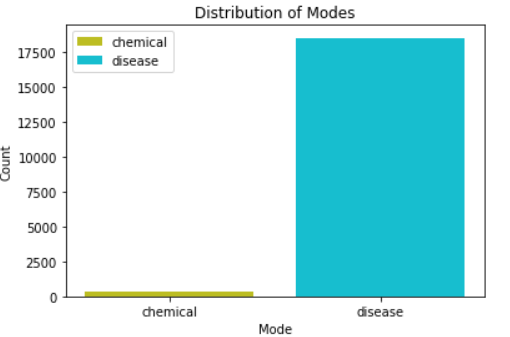
\includegraphics[width=\linewidth]{Modes.png} 
\caption{Mambo Modes Creation Overview}
\label{fig:mambo_architecture} % Label for referencing the image within your text
\end{figure}



\\
\begin{figure}[htbp]
\centering
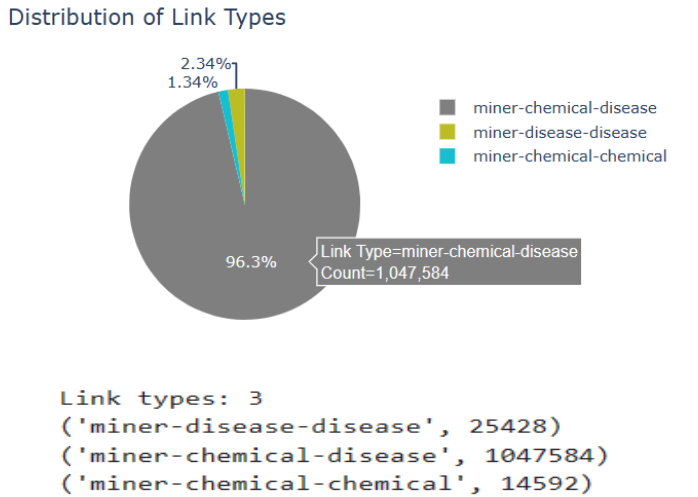
\includegraphics[width=\linewidth]{LinkeTypesCreation.png} 
\caption{Link Types Creation Overview}
\label{fig:mambo_architecture} % Label for referencing the image within your text
\end{figure}
Mambo has constructed Modes for group of chemical which are also known as drugs according to Drug Bank and other sources and the meaning is same. Other than the Half-Life Prediction, the project requires only two types of data which contains chemical, disease and the entities count individually are 359 for chemcial and 18,554 for disease. 

Once the Modes are created, Mambo focuses on Link Types or Relationships or Edges to specify the relationships between Modes and these relationships are formed using Mapping Tables to make the nodes to group similar modes without any issues caused by different terminologies used by BioMedical data providers. 



The primary methodology for this project centers on a graph-based analysis of drug interactions. In this network model, drugs and their potential side effects are represented as interconnected nodes. This graphical representation facilitates an in-depth analysis of the complex relationships between drugs and their side effects. Feature extraction, a key step in the process, leverages graph-related techniques to capture essential properties of drugs and their interactions. These features are crucial for building predictive models based on Graph Machine Learning, that can assess the likelihood of a drug combination resulting in an ADR or DDI. Below figure 2 briefly explains the architecture the team has employed while working on the ADR prediction problem for various DDIs.

\begin{figure}[htbp]
\centering
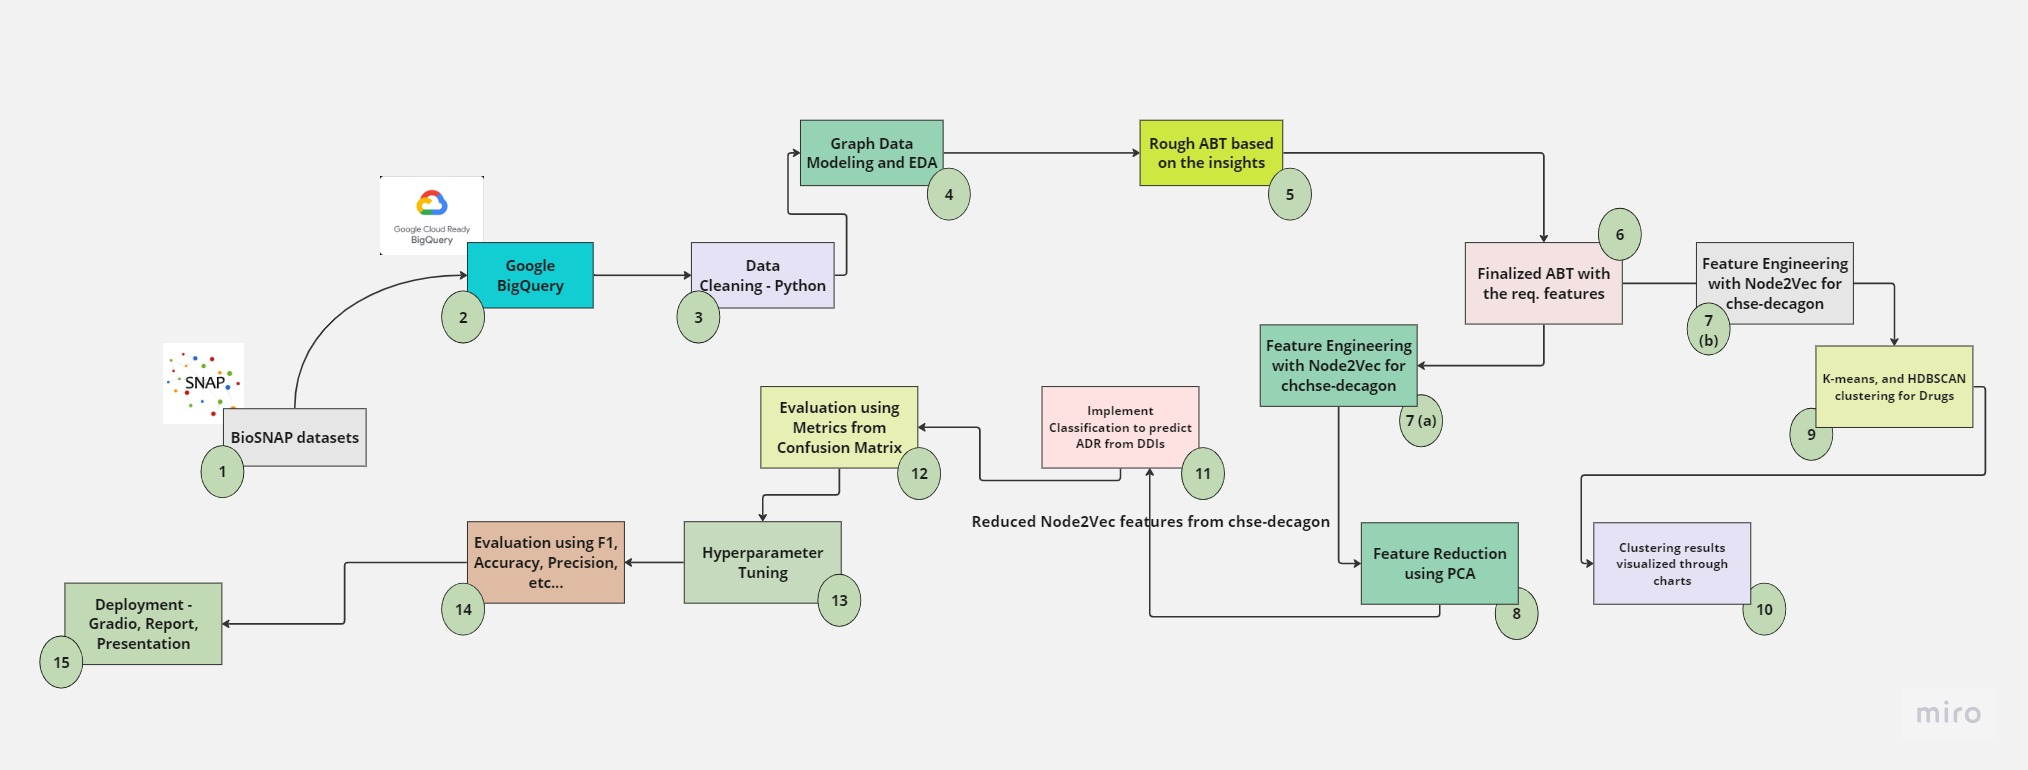
\includegraphics[width=\linewidth]{primary_architecture.jpg} 
\caption{Architecture for Graph Data Modeling and Prediction of DDR against various DDI}
\label{fig:primary_architecture} % Label for referencing the image within your text
\end{figure}

From the above Fig.4. it can be followed that the study starts with acquiring the BioSNAP datasets from their homepage, and do upload them directly to BigQuery, as BigQuery is a columnar db, getting the data into database was pretty straight forward. Once the data was in the database, the team executed some SQL queries to understand the relationships of the data, as they were graph datasets, which means they are long and thin. The next step was to pull this data into Python using Google BigQuery Python connector, The team applied general data cleaning techniques, and uploaded the cleaned datasets back into BigQuery DB. As these datasets are Graph datasets, meaning there are very few features, like drug\_a, drug\_b, and side-effects associated with the drug-drug interaction. The next step was to do some EDA specific to the Graph datasets that were being employed. For Feature Extraction, this project banks on the Node2Vec feature extraction technique which is prominent in NLP, but can also be leveraged for Graph datasets. Node2Vec features are first normalized using standardscaler, PCA and T-SVD are experiemented for Dimension reduction techniques, as Node2Vec creates 128 dimensions for each node (Drug), based on the graph structure, generating random walks across the graph to understand the structure, connected edges and various other distance metrics. Post dimension reduction, the reduced Node2Vec feature set for chse-decagon is used for Clustering the similar drugs based on the assoicated side-effects. Using elbow method, an optimal 'k' is employed to divide the drugs into specific cluster. K-means, and HDBSCAN algorithms are experimented with, and the results are shared in further sections. Reduced Node2Vec feature set for chchse-decagon dataset is further scaled, balanced, and then split for test, train and valid datasets, and passed into various classifiers like Random forest, Logistic regression, SGD Classifier, and finally Graph Neural Networks classifer to decide whether a particular DDR results in an ADR or not. Post hyperparameter tuning employing GridsearchCV, Gradio is utilized to deply the classifier models, and show the real time classification results with the experimented models.

\\
Ultimately, this study seeks to provide healthcare professionals with valuable tools for informed decision-making regarding drug prescriptions in polypharmacy scenarios. By accurately predicting potential ADRs and DDIs, these tools aim to significantly reduce the incidence of medication-related complications, thereby improving patient safety.  These tools will contribute to the field of pharmacovigilance by enhancing the understanding of drug interactions, thus improving the monitoring, reporting, and management of medication safety. The importance of this study lies in its potential to revolutionize how medications are prescribed in scenarios of polypharmacy. By mitigating the risks associated with ADRs and DDIs, it aims to not only enhance medication safety but also to significantly improve patient care outcomes. The application of these tools in healthcare settings has the potential to transform the management of polypharmacy, making it a safer and more effective practice.

\subsection{Process Model}
As this domain was completely new to the team and its a Data Science/Machine Learning Project, CRISP-DM methodology was employed across the project, as it gives the team to be flexible with the problem statements being pursued. Initially the idea was to work around a Multi-class side-effects prediction problem, but due to the computational and technical challenges, the team had to revert back to Business Understanding. This was only possible due to the crisp-dm methodology that is being followed sincerely. All the six phases and various work-items of this CRISP-DM methodology are detailed below:

\begin{figure}[htbp]
\centering
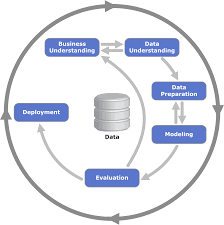
\includegraphics[width=5 cm]{crisp-dm.png} 
\caption{CRISP-DM Methodology for the Project}
\label{fig:crisp-dm methodology} % Label for referencing the image within your text
\end{figure}

\begin{enumerate}
    \item Business Understanding: During this phase, the team discussed various project ideas of interest, with respect to the given domain, i.e... Network data and as per the suggestions, the team explored BioSNAP and SNAP datasets, and shortlisted top 3 problem statements, out of which this Polypharmacy prediction usecase has been finalized. Post finalizing the project topic, Each individual of the team has made their own literature survey to understand various components of this project like what is the existing research, scope of work, technologies that can be used, How much domain knowledge and Subject Matter Expertise does this project needs, and whether it has all the data that would be required for modeling and other ML usecases, all of these components were evaluated as a team post literature surveys.
    \item Data Understanding: During the Data Understanding phase of this project, the team focused on comprehending the Drugbank dataset, accessed via a data pipeline using REST APIs from the DrugBank database. Additional primary datasets, including chchse-decagon and chse-decagon, were sourced from the BioSNAP homepage. This phase also involved comprehensive exploratory data analysis to determine the appropriate graph modeling techniques for these graph datasets. Data cleaning and transformation procedures were established as a result of this phase. A critical aspect was assessing the feasibility of multi-label classification for predicted side-effects. After evaluation, the team concluded that this approach would be computationally intensive and thus, infeasible. Consequently, they revisited their strategy to align with the project's constraints and resources.
    \item Data Preparation: During this phase, various pre-processing activities were undertaken, including data cleaning, identifying and addressing outliers, and feature selection for both the sentiment analyzer classifier and the K-Means model. As the primary datasets are graph datasets, it was really important to understand the feature extraction techniques which were compatible with K-means, and Binary classification.Similary, DrugBank dataset for Half-Life Prediction is also undergone the same approach used by BioSNAP dataset Since the datasets are from Pharmacetical Knowledge database and features are extracted by using random forest regression to get the important features and generated ABT table.
    \item Modeling: In the modeling phase, Major development was taken care of. Elbow method was employed to get the optimal 'K' and the drug clusters were created. Various Machine learning models were implemented for the Binary classification problem, such as Random Forest, Logistic regression, SGD, and Graph Neural Networks. The team developed models for both the side-effect classifier and the K-Means algorithm. Following the implementation of these models, they conducted a thorough evaluation of the results. To refine and optimize the models, techniques such as cross-validation and hyper-parameter tuning were employed. Specifically, for hyper-parameter tuning, the Random Search CV method was utilized to identify the most optimal parameters for the models, aiming to create an effective recommender system. In Half-Life Prediction modeling, Random forest regression is used to identify the Half-Life of a pill and tuned the hyperparameters.
    \item Data Evaluation: In this stage, the team compared the accuracy of each model against the others. These models were executed using a range of performance metrics like confusion matrix, F1-score, etc... The primary objective behind utilizing diverse models was to determine which method yielded the highest accuracy. This process was crucial in enhancing the accuracy of the models, ultimately aiding the team in developing a highly precise proposed system. Out of all the other models, Graph Neural Networks performed very well with an accuracy close to ~87\% which is quite good for any good solution. Another Model on Half-Life prediction uses MAE,MSE,R2 and Training Time evaluation metrics to evaulate the model and predictions are not accurate as expected though the model is hyperparameterised and Future scope for further enhancement of adopting better models.
    \item Deployment: Finally, after the models and results are ready, the front-end was created employing gradio python libraries. This scalable library offers a range of built-in functions to develop an interactive and advanced front-end interface. Following the front-end development, it was seamlessly integrated with the machine learning model to facilitate result prediction.
\end{enumerate}

\begin{table}[htbp]
\centering
\caption{Datasets employed in this Project}
\label{tab:Datasets description}
\begin{tabular}{|c|c|c|c|}
\hline
S.No & Dataset Name & Description \\ \hline
1 & chchse-decagon & Side effects of DDI \\ \hline
2 & chse-decagon & Drug, side-effect network \\ \hline
3 & side-effect categories & side-effects classes \\ \hline
4 & DrugBank & drugs and half-life combinations \\ \hline
\end{tabular}
\end{table}


\section{DATA PREPARATION}
This phase of CRISP-DM methodology involves conducting Exploratory Data Analysis, Data pre-processing, Data transformation and data preparation for the model. In this project, this was one of the most important phases for this project, as the datasets that were employed for the course of project, and specific usecases needed a lot of pre-processing to change them into formats that were suitable for modeling. The data preparation steps that were involved in this project were Data cleaning, Dropping null columns, imputing null values with suited statistical techniques, merging datasets, filtering of the data, Data transformation to change the schema to suit for the specific modeling technique, converting graph features into numerical vectors, Dimensionality reduction, and splitting the dataset into testing, and training. The unique functionality of this project was, the team had to do the pre-processing with distinct methods for datasets chosen. Each dataset had a specific use-case, so there are significant changes in the way the data is prepared for the modeling phase. Below figure 4 shows the data flow diagram for the Data preparation flow for the chse-decagon dataset which was extracted from BioSNAP datasets.  

\\
\begin{figure}[htbp]
\centering
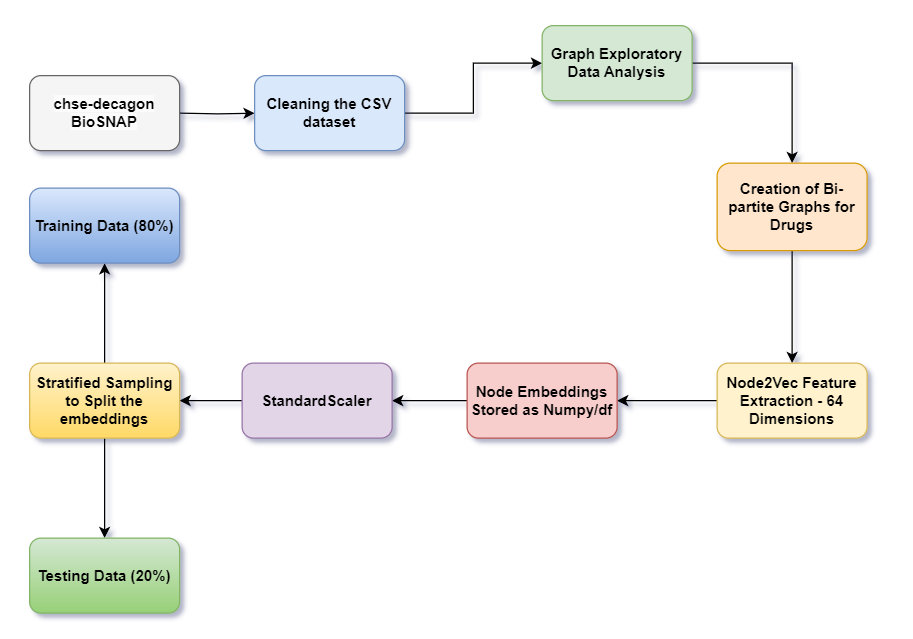
\includegraphics[width=\linewidth]{data_flow_chsedecagon.PNG} 
\caption{Data Flow Diagram for the chse-decagon BioSNAP dataset}
\label{fig: Chse-decagon data flow diagram} % Label for referencing the image within your text
\end{figure}

The difference between the data preparation steps for chse-decagon, and chchse-decagon dataset is how these datasets are being employed for this research. The former dataset will be utilized to build Bi-partite graphs for both Drugs, and side-effects as separate nodes, and these bi-partite graphs will be used for clustering, where similar drugs are grouped together based on the intensity of the edges, which means two drugs are connected if they share a common side-effect, this computation is not done for side-effects as they are very densely connected, and the number of nodes are quite high, meaning the complexity of creating the graph, and other preparation techniques would be difficult to employ for a side-effect bi-partite graph. The later, chchse-decagon has a different use-case in this research, which is to help understand whether a DDI causes an ADR or not. This classification problem needs a data transformation, to convert the existing chchse-decagon schema to a schema which is suitable for binary classification, this is explained in further pre-processing sections. Figure 5 gives the data flow diagram for chchse-decagon BioSNAP dataset. 

\begin{figure}[htbp]
\centering
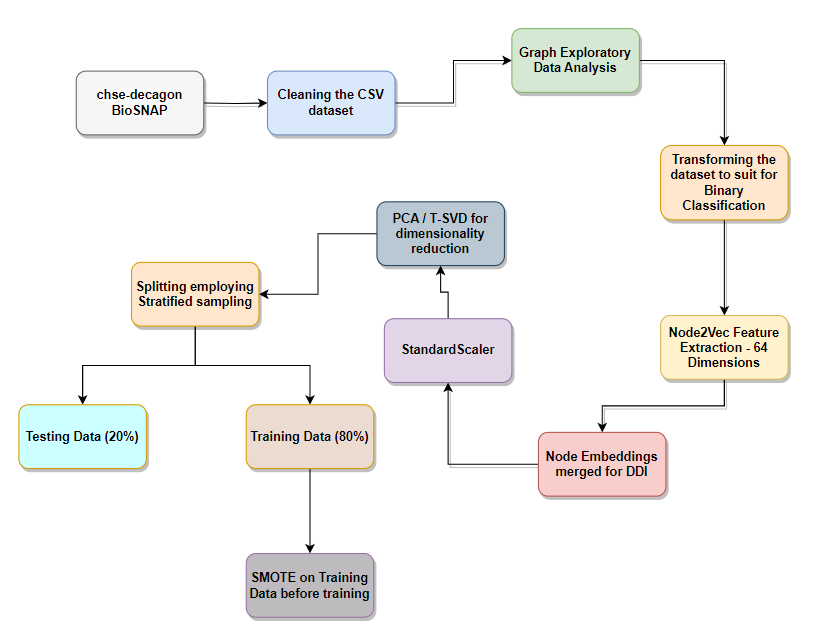
\includegraphics[width=\linewidth]{dataflow_chchse.PNG} 
\caption{Data Flow Diagram for the chchse-decagon BioSNAP dataset}
\label{fig: chchse-decagon data flow diagram} % Label for referencing the image within your text
\end{figure}

\begin{figure}[htbp]
\centering
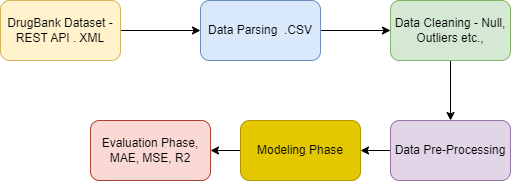
\includegraphics[width=\linewidth]{ML DataFlow Diagram.drawio.png} 
\caption{Data Flow Diagram for the DrugBank dataset}
\label{fig: chchse-decagon data flow diagram} % Label for referencing the image within your text
\end{figure}

Here, The data is collected from DrugBank using REST API by accessing the endpoint and then the data is in .XML format and that needs to be parsed to make the file type as .CSV and then data needs to be cleaned similar to BioSNAP datasets and Data Pre-Processed to make the data compatible with the model without changing the characteristics of the Drug Bank data and then model is evaluated to predict the accuracy. 

\subsection{Data Exploration}
The first step of Data Exploration was to understand how to model the BioSNAP datasets. This is a very important phase in this project due to the fact that this research is majorly based on the Graph BioSNAP datasets. In Graph Modeling, each drug is depicted as a Node, and side-effects are modeled as associations between these drugs. chse-decagon dataset has a many to many mapping between 'Drug' and 'Side effect', meaning one drug can cause multiple side-effects, and one side-effect can be caused by one or more than one drug. chchse-decagon dataset has a similar representation, but each DDI has numerous side-effects associated in between them, making this a really complex graph to understand with Multi-labels for a particular instance. Below is figure 6 where Graph data model for the BioSNAP datasets is illustrated. 

\begin{figure}[htbp]
\centering
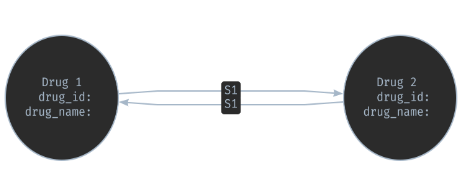
\includegraphics[width=\linewidth]{chse-decagon-graph.PNG} 
\caption{Graph Data Model for chse-decagon dataset}
\label{fig: chse-decagon sample Graph Data Model} % Label for referencing the image within your text
\end{figure}

The above Graph data model, makes sure to connect two drug nodes, if there exists a side-effect association between them, Similar Graph data modeling is also employed with chchse-decagon dataset, which is illustrated below, in figure 7, this sub-graph is extended towards other nodes, and side-effects are still modeled as associations between the side-effects. Multiple side-effects for single DDI are modeled as properties of the edges in this graph model for chchse-decagon. 

\begin{figure}[htbp]
\centering
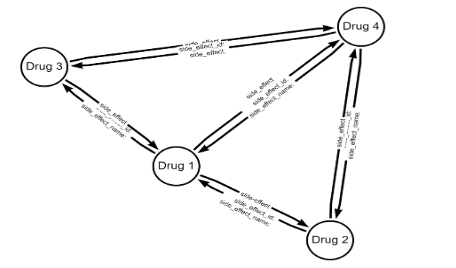
\includegraphics[width=\linewidth]{chchse-decagon-graph.PNG} 
\caption{Graph Data Model for chchse-decagon dataset}
\label{fig: chchse-decagon sample Graph Data Model} % Label for referencing the image within your text
\end{figure}

The objective behind this Exploratory Data Analysis is to understand the complexities of the Graph Data Models which were created. Respective graphs using Networkx were created for both the BioSNAP datasets. The next step was to compute some graph related metrics to understand the graphs. One such metric which easily helped us to identify the complexity, was to look at the Degree distribution of both the bi-partite projections that were created from chse-decagon dataset. Below is figure 8 which gives the number of nodes and edges 

\begin{figure}[htbp]
\centering
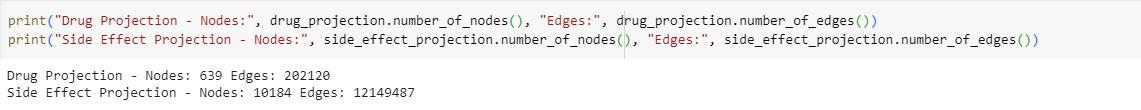
\includegraphics[width=\linewidth]{bi-partite-projection-chse.PNG} 
\caption{Stats from Bi-partite graph projections of Drugs, Side-effects from chse-decagon}
\label{fig: chse-decagon bi-partite details} % Label for referencing the image within your text
\end{figure}

The above numbers from bi-partite graph suggest that its compute easy to prepare and model the bi-partite projection of Drugs.

Below is Figure 9, which visualizes the degree distribution from the side-effect Projection from chse-decagon, degree distribution plot gives us the frequency against degrees (connectivity) for Side-effect projections. 

\begin{figure}[htbp]
\centering
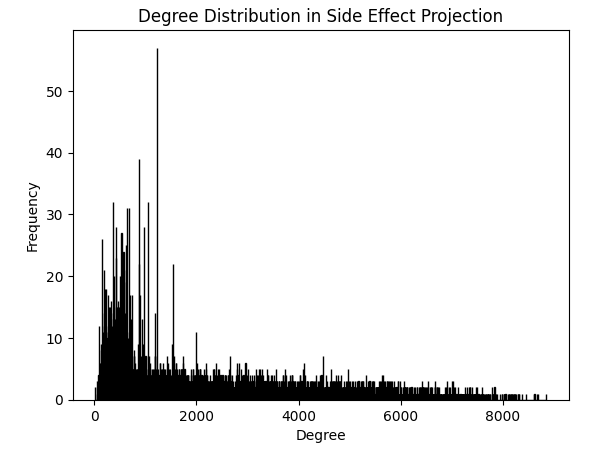
\includegraphics[width=\linewidth]{degree_projection_se_bipartite.PNG} 
\caption{Degrees of each side-effect (Node) vs Frequency in the side-effect projection of chse-decagon}
\label{fig: chse-decagon side-effect bi-partite details} % Label for referencing the image within your text
\end{figure}

The above degree distribution plot shows that frequency of the value of degree, in side-effects projection is significantly distributed, resulting in compute heavy, complex, and time taking operations while working with the dataset, making it really hard to prepare the data for Modeling phase. Below figure 10 shows the clustering co-efficient and other important metrics of the Drugs projection, to understand whether its worth it to go ahead with the clustering for Drug projection or not. 

\begin{figure}[htbp]
\centering
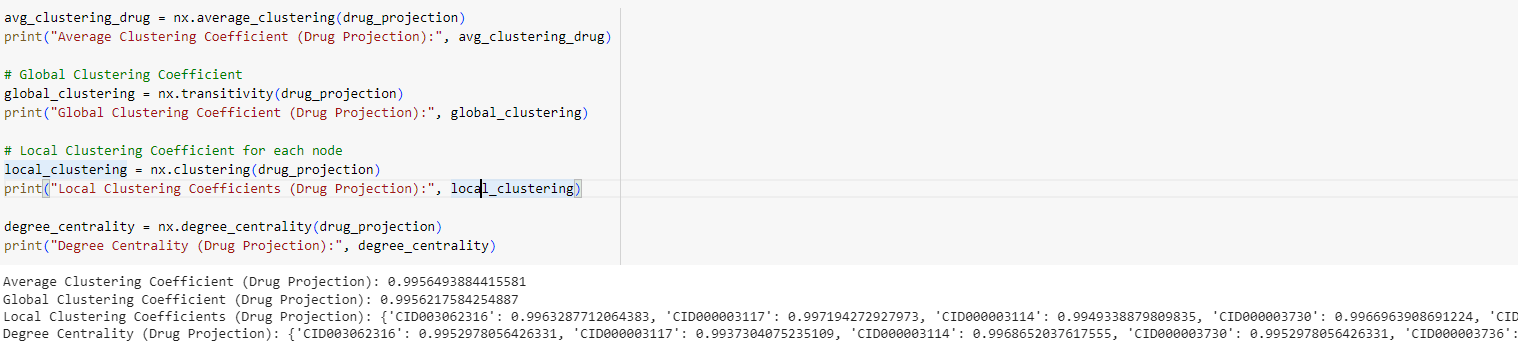
\includegraphics[width=\linewidth]{graph-metrics-drug-projection.PNG} 
\caption{Clustering metrics for Drug projection of chse-decagon dataset}
\label{fig: chse-decagon drug projection clustering metrics} % Label for referencing the image within your text
\end{figure}
Observations followed from the above clustering numbers - In simpler terms, if a node A is connected to node B and node C, there's a very high probability that nodes B and C are also connected to each other. Such a high clustering coefficient often suggests that the network has a strong tendency to form local clusters or groups. In the context of a drug interaction network, a high clustering coefficient might suggest that drugs tend to have side effects in common with many other drugs they interact with. This could be indicative of a network where many drugs share similar pharmacological properties or side effects, confirming that Drug projection can be used for Clustering.
\\

For chchse-decagon, which comprises roughly 4.2 million rows only with 4 columns, 'drug\_a', 'drug\_b', 'side\_effect\_id' and 'side\_effect\_name'. Below Figure 11 displays the number of nodes, and edges this Graph dataset is going to create when constructed as a graph. The mapping between DDI and Side-effects is one to many, as a single DDI can cause multiple side-effects and vice-versa. Visualizations from figure 10 below, explain how the network structure indicated by these centrality measures points towards a relatively sparse network with a limited number of highly central drugs. This suggests that a binary classification approach might be more feasible and efficient for predicting drug interactions, especially if the dataset is large and the interactions between drugs are not densely interconnected. Binary classification would simplify the model and reduce the computational complexity by focusing on the presence or absence of an interaction rather than predicting multiple potential interactions for each drug pair. 

\begin{figure}[htbp]
\centering
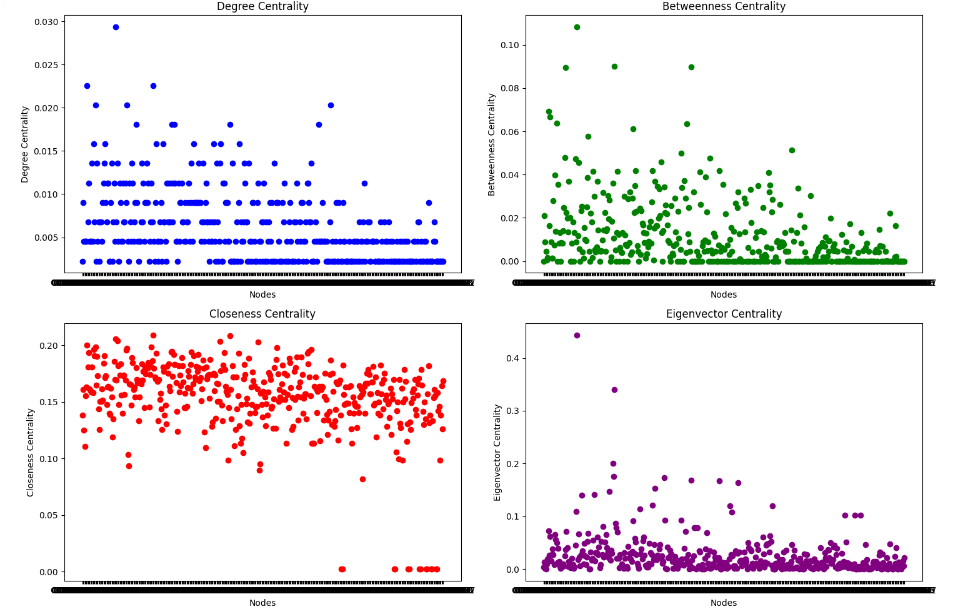
\includegraphics[width=\linewidth]{chchse-decagon-graph-metrics-viz.PNG} 
\caption{Graph Metrics to Understand the characteristics of the chchse-decagon dataset}
\label{fig: chchse-decagon visualization metrics } % Label for referencing the image within your text
\end{figure}

Overall, these metrics suggest a network where drugs are moderately interconnected without a strong dependency on a small set of highly influential drugs. The network exhibits a decent level of integration, with no single or small group of drugs dominating the connectivity or influence within the network, the below average metrics of the chchse-decagon dataset, confirm the theory to navigate towards a Binary classification problem. 

\begin{figure}[htbp]
\centering
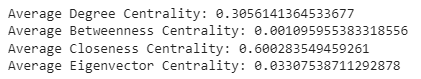
\includegraphics[width=\linewidth]{chchse-decagon-graph-metrics.PNG} 
\caption{Avg Graph Metrics extracted from the chchse-decagon dataset}
\label{fig: chchse-decagon visualization metrics } % Label for referencing the image within your text
\end{figure}

\begin{figure}[htbp]
    \centering
    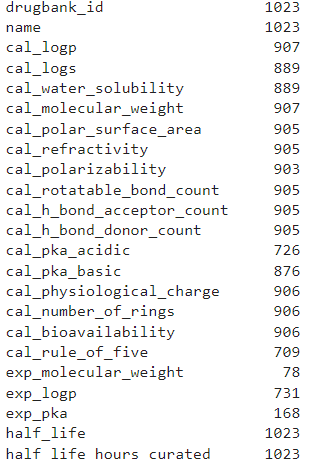
\includegraphics[width=0.4\linewidth]{Data Exploration_Main.png} % Adjust the width value as needed
    \caption{DrugBankDataset Overview and its column rows count}
    \label{fig:chchse-decagon visualization metrics}
\end{figure}
\\
The provided metadata pertains to drug compounds, encapsulating various properties either extracted or calculated for each compound. Each field within the metadata serves a distinct purpose, such as the drugbankid, a unique identifier in the DrugBank database, and the name, denoting the nomenclature of the drug compound. Additionally, calculated properties like logP, water solubility, molecular weight, polar surface area, and others provide insights into the drug's lipophilicity, solubility, structure, and pharmacokinetic characteristics. Notably, parameters like pKa values, hydrogen bond counts, and adherence to the "Rule of Five" contribute to understanding the drug's chemical behavior. Experimental measurements, including molecular weight, logP, and pKa, complement the dataset, along with details on the drug's half-life, curated and validated in hours.

In summary, these metadata fields collectively present a comprehensive overview of the chemical, physical, and pharmacokinetic attributes of the drug compounds, offering valuable insights for research and analysis.


\subsection{Data Pre-processing}
The primary objective is to conduct the pre-processing on the BioSNAP datasets, and clean the Drugbank dataset. Cleaning the drugbank dataset will be discussed in the later part of this subsection. For chse-decagon BioSNAP dataset, the pre-processing steps include creating a new Drug Bi-partite graph, which only has Drugs as nodes, and two drugs are only connected if they have common side-effects. The bi-partite graph of  Drug Projection is shown in below figure 13.

\begin{figure}[htbp]
    \centering
    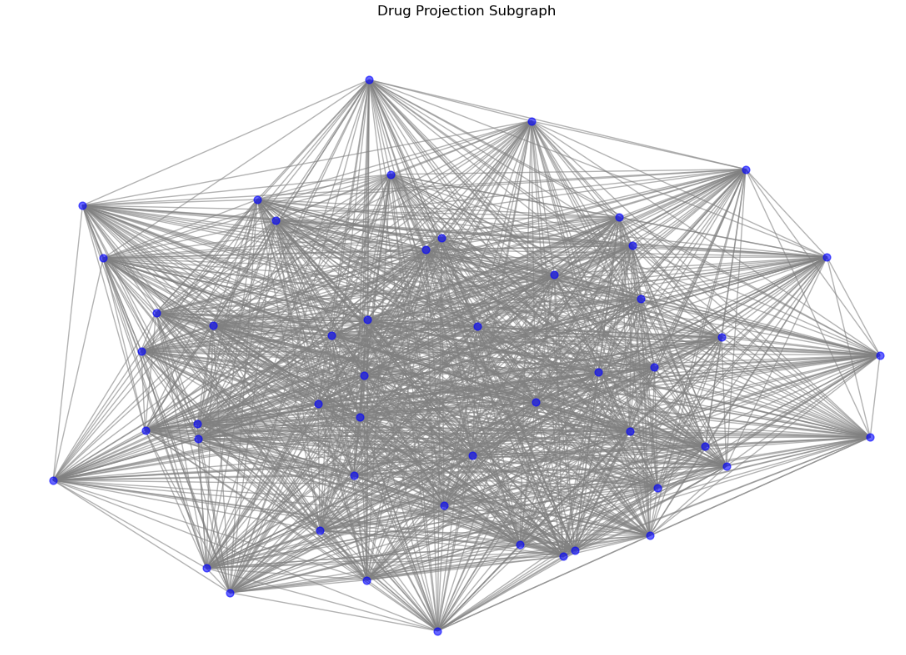
\includegraphics[width=0.8\linewidth]{bipartite_graph_drugs_chse.PNG} % Adjust the width value as needed
    \caption{Drug Bi-partite graph from chse-decagon}
    \label{fig:chse-decagon-drugs-bipartite-graph}
\end{figure}


The above created drug bi-partite graph is stored in the form of graph object for further feature extraction techniques. It can be observed from the Visualization, that the Drugs (nodes) are tightly knit, making it a solid use-case for clustering with numerous applications. For chchse-decagon dataset, this pre-processing phase is really crucial, as the team has decided to move on with the binary classification, after multiple failed attempts of working on the Multi-class classification problem which was really interesting and very common to this kind of Graph dataset. The pre-processing that's required for chchse-decagon dataset is to convert into a tabular schema which can be used for Binary classification of the predicted sideeffects. This pre-processing is done through Python, below is an example of how the schema changed due to this pre-processing. Figure 14 illustrates this pre-processing step for chchse-decagon dataset.

\begin{figure}[htbp]
\centering
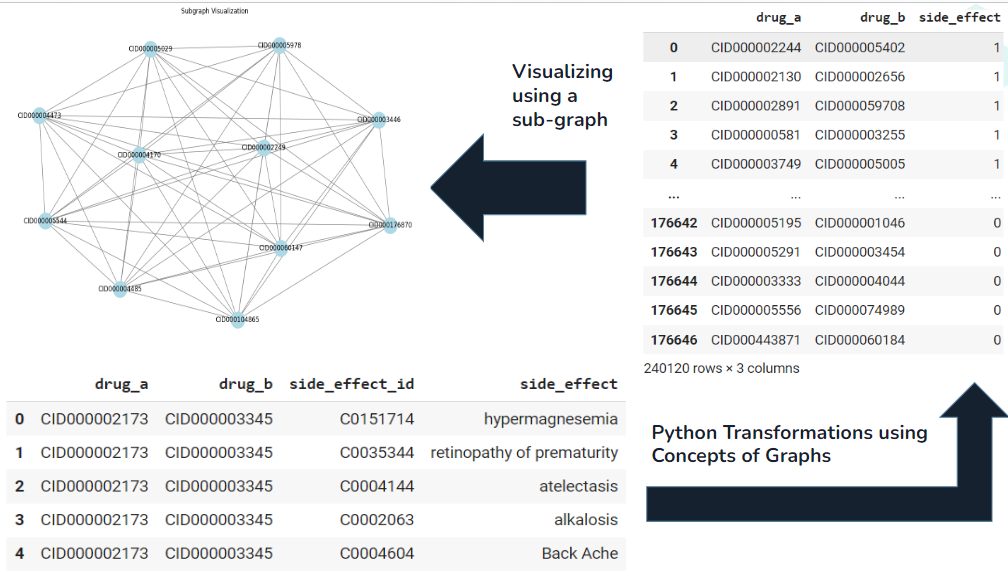
\includegraphics[width=\linewidth]{chchse-decagon-preprocessing.PNG} 
\caption{Preprocessing the chchse-decagon for Binary Classification}
\label{fig: chchse-decagon Binary classification dataset} % Label for referencing the image within your text
\end{figure}

The transformation effectively balances the dataset with an equal representation of drug pairs with and without side effects, which is crucial for binary classification tasks to prevent model bias towards the more frequent class.


\begin{figure}[htbp]
\centering
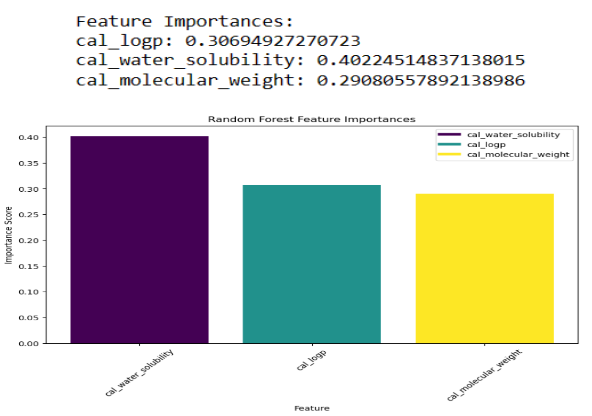
\includegraphics[width=\linewidth]{Data PreProcess 1 Feature Importance.png} 
\caption{Preprocessing the DrugBankDataset to get feature importance}
\label{fig: chchse-decagon Binary classification dataset} % Label for referencing the image within your text
\end{figure} 

\\
For DrugBank Dataset, Finding the Feature importance using random forest regression to provide the features to the Half-Life Prediction model for better accuracy. Finally, Built the ABT table for Half-Life Prediction.



\subsection{Data Transformation}
The most important phase for the entire machine learning adaptation of the defined problem statement is here. To apply machine learning algorithms and models, the first and foremost requirement is data, i.e... features, and ML-required problem statement. This problem statement has a well defined problem statement with lots of real-time applications, what its missing is input features. As the graph datasets are typical examples of Long and Thin datasets, due to their modeling on relationships rather than the individual data points, there are almost no features we can directly use from the datasets, and there isn't much reliable pharmaceutical information to use them as features. The way to get out of this situation is to employ Node2Vec. 

Node2Vec is an algorithmic framework for learning continuous feature representations for nodes in networks. It was introduced by Aditya Grover [6] in their paper "node2vec: Scalable Feature Learning for Networks," presented at the KDD 2016 conference. The algorithm is designed to capture the diversity of connectivity patterns in a network, enabling a wide range of machine learning applications. Node2Vec operates on the principle of preserving network neighborhoods of nodes. It does so by efficiently exploring diverse neighborhoods by employing a biased random walk procedure, which balances the exploration between breadth-first sampling (BFS) and depth-first sampling (DFS). This approach allows Node2Vec to learn representations that encode both local and global network structures. The random walks are guided by two parameters, p and q, which control the likelihood of immediately revisiting a node and exploring the graph away from the starting node, respectively. This enables the balance between BFS-like and DFS-like neighborhood exploration. The sequences of nodes visited in the random walks are treated as sentences in a language model. The algorithm then uses techniques similar to those used in word2vec (specifically, the Skip-gram model) to learn node representations by maximizing the likelihood of preserving node neighborhoods. For bipartite graphs like drug projection graphs, which consist of two types of entities (e.g., drugs and side effects), Node2Vec can learn to represent the relationships between these entities. This can be particularly useful when trying to project one type of entity onto the other, to understand their interactions at a higher level. In the context of DDIs and ADRs, Node2Vec can help learn representations for drugs that not only reflect their interactions with other drugs but also their potential to cause adverse drug reactions. This could enable more effective prediction of new DDIs and ADRs by learning the complex patterns that lead to such events. Node2Vec's ability to learn rich feature representations makes it particularly useful for tasks such as clustering, classification, and prediction within network datasets. In the field of pharmacology, where understanding the complex relationships between different entities is crucial, Node2Vec's nuanced approach to feature learning can provide valuable insights that might not be captured by simpler graph analysis techniques.

\begin{figure}[htbp]
\centering
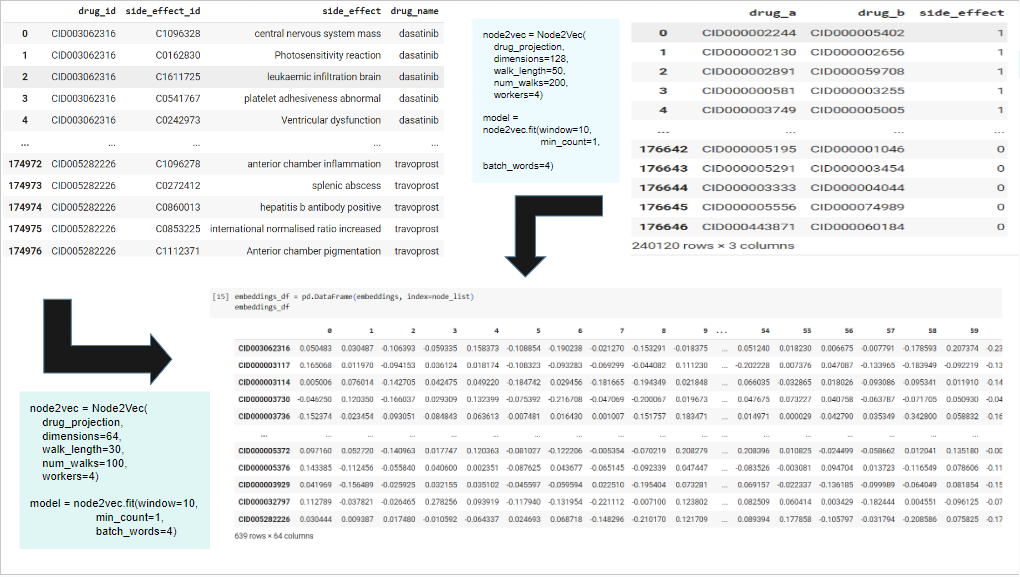
\includegraphics[width=\linewidth]{Node2Vec_biosnap.PNG} 
\caption{In the above transformation step, Node2Vec has been applied to both the Drug projection (chse) and the transformed binary classification (chchse), for the sake of space they are shown to be the same, but these features are extracted separately as the usecases are different} 
\label{fig: Node2Vec Feature Extraction technique} % Label for referencing the image within your text
\end{figure}
For chse-decagon Drug projection, 64 dimensions, and the other Parameters employed while applying Node2Vec should provide satisfactory results. When it comes to classification problem, the prediction is being done on a DDI rather than a single drug, so both the sets of 64 Dimensions, for each set of nodes (drug\_a, drug\_b), resulting in a total of 128 columns which is shown the below figure 16. 
\begin{figure}[htbp]
\centering
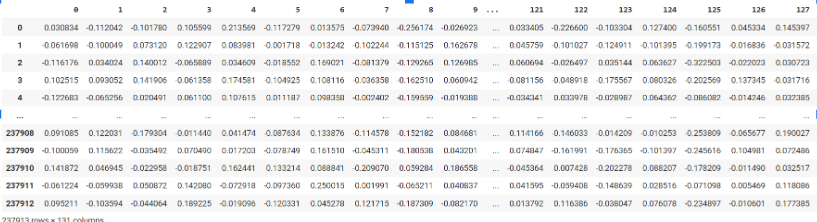
\includegraphics[width=\linewidth]{node2vec-chchse.PNG} 
\caption{Above is the transformed dataset for DDI-ADR prediction problem} 
\label{fig: Node2Vec Feature Extraction technique for chchse} % Label for referencing the image within your text
\end{figure}
Post feature extraction from BioSNAP datasets, a round of scaling is usually preferred to make sure the vectors are normalized. As a next step, the team have split the feature sets into 80-20, train and test split, this is done by employing stratified sampling with sklearn, post splitting the data into training, SMOTE is applied to balance the positive classes which were initially much less than the negative (no side-effect). Then, as a next step the team tried to experiment with the dimensionality reduction techniques like PCA and T-SVD. The idea is not to vary the variance by far, so that the Node2Vec extracted feature vectors still capture the essence of the graph dataset they were extracted from. The idea behind employing a dimension reduction technique here is to decrease the training time, while trying to improve the performance of the model, without changing the variance too much. Below Figure 17 is the variance against number of components plot for Binary classification Node2Vec (128) features.  
\begin{figure}[htbp]
\centering
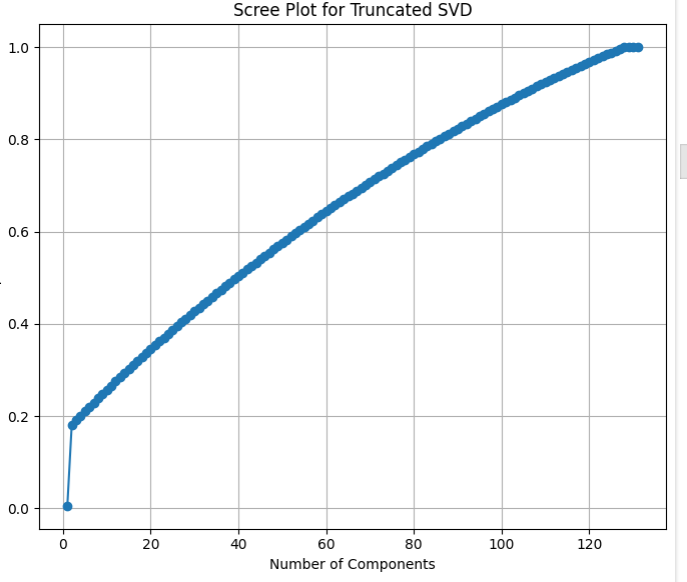
\includegraphics[width=\linewidth]{TSVD-chchse.png} 
\caption{Variance against number of components plot for Binary classification} 
\label{fig: T-SVD for binary classification} % Label for referencing the image within your text
\end{figure}
From the above distribution, to capture a variance greater than or equal to 80\%, the number of reduced components are 80 and greater. Based on the level of variance that can be retained, the number of components can be chosen, and vice-versa. Its a trade off basically, trading off training time for complete n\_components. 
Below is the table figure 18 to capture the variance and reduced components for TSVD,
\begin{figure}[htbp]
\centering
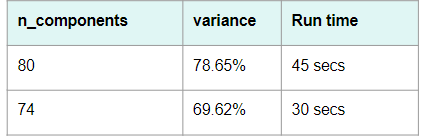
\includegraphics[width=\linewidth]{svd-table.PNG} 
\caption{Comparing the best training times while employing SVD} 
\label{fig: SVD variance and time} % Label for referencing the image within your text
\end{figure}
From the above table figure 20, it can be seen that variance is directly proportional to variance, which is directly proportional to the run time. 
\begin{figure}[htbp]
\centering
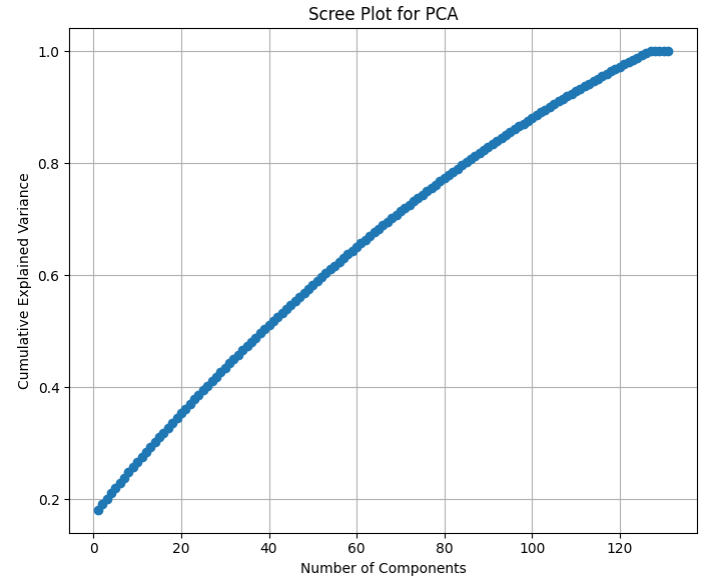
\includegraphics[width=\linewidth]{PCA-chchse.png} 
\caption{PCA Variance against number of components plot for Binary classification} 
\label{fig: PCA for binary classification} % Label for referencing the image within your text
\end{figure}
From the above distribution, to capture a variance greater than or equal to 80\%, the number of reduced components are 75 and greater. The trade-offs are similar when compared to T-SVD. 
Below is the table figure 21 to capture the variance and reduced components for PCA,
\begin{figure}[htbp]
\centering
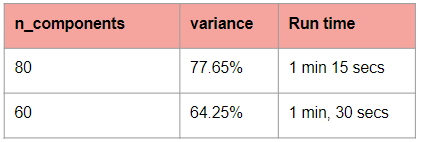
\includegraphics[width=\linewidth]{pca-table-chchse.PNG} 
\caption{Comparing the best run times while employing PCA} 
\label{fig: PCA variance and time} % Label for referencing the image within your text
\end{figure}
From the above comparison with T-SVD, the run times are better, the time difference may be very minute now, but with huge amount of data its always going to scale out. 

\section{Modeling}
For Modeling, the Node2Vec extracted 64 dimensions feature set is used as input features. K-means is a clustering algorithm that partitions n observations into k clusters in which each observation belongs to the cluster with the nearest mean. This is particularly suitable for the vectors generated by Node2Vec because:
\begin{itemize}
    \item \textbf{Node2Vec} first captures the local and global structures within the graph, reflecting these as feature vectors that encode the similarities and differences between nodes based on the graph's topology (in this case, shared side effects).
    \item \textbf{K-means} then groups these feature vectors into clusters, allowing us to discern distinct groups of drugs that share similar profiles in terms of how they interact with others and the side effects they may cause.
\end{itemize}
For a k-means clustering algorithm, as the initial value of k can be user-defined, the team started with 5, below figure 22 illustrates the set of clusters that k-means could come up with.
\begin{figure}[htbp]
\centering
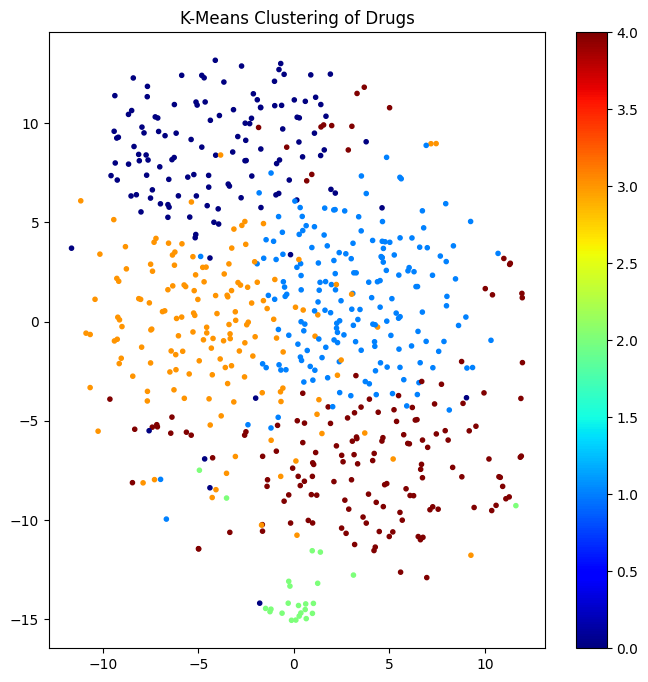
\includegraphics[width=\linewidth]{kmeans_initial.png} 
\caption{K-means with experimentation (k=5)} 
\label{fig: Initial K-means clustering} % Label for referencing the image within your text
\end{figure}
There are significant number of data points which overlap or wrongly belong to other clusters. To get the optimal values of k for the feature set, the team implemented Elbow-method to understand the optimal 'k'. The Elbow Method is a technique to determine the optimal number of clusters for k-means clustering. It involves running k-means multiple times with different numbers of clusters (k) and plotting the within-cluster sum of squares (WCSS) against k. The point where the WCSS starts to decrease at a slower rate, resembling an "elbow" on the graph, is considered the best value for k. This point represents a balance between having too few and too many clusters, minimizing both the within-cluster variance and the complexity of the model. The Elbow Method is subjective and is often used with other methods to validate the choice of k. Below figure 24 shows the elbow is at k=3.
\begin{figure}[htbp]
\centering
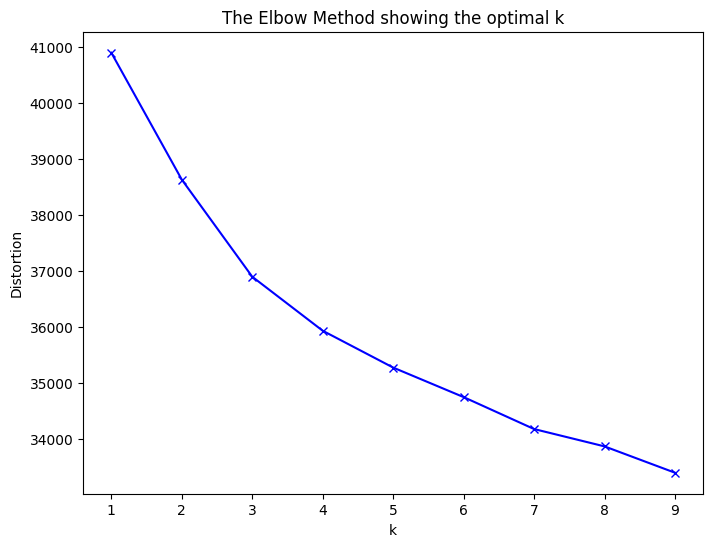
\includegraphics[width=\linewidth]{elbow_for_kmeans.png} 
\caption{Elbow method for finding Optimal 'k'} 
\label{fig: Elbow method for K-means} % Label for referencing the image within your text
\end{figure}
Now using optimal 'k' value from the elbow method which is 3, and re-fitting the K-means would give us the clusters, based on the drug connectivity, graph structure captured through Node2Vec features. Below figure 25 is the hypertuned K-means clustering, the noise is reduced and the clusters are mostly distinct with the optimal value of K used. 
\begin{figure}[htbp]
\centering
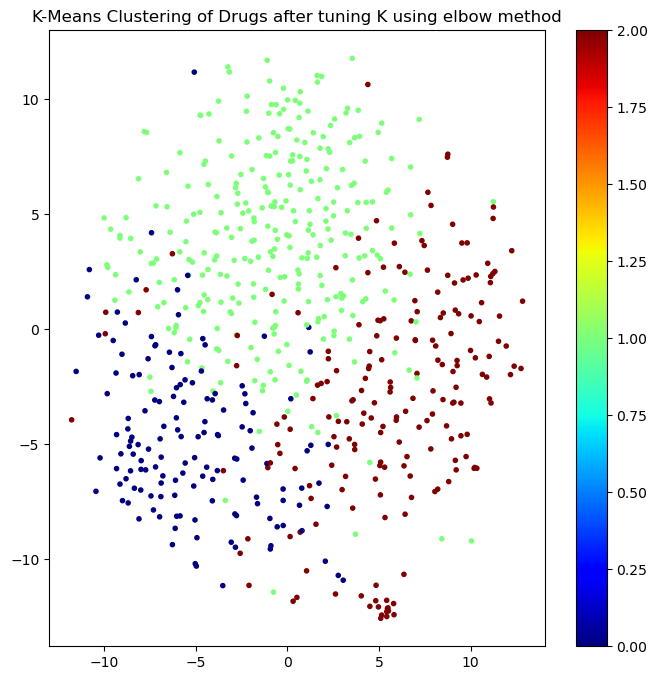
\includegraphics[width=\linewidth]{k-means-after-k.png} 
\caption{K-means clustering results after Hypertuning} 
\label{fig: K-means after setting the optimal k} % Label for referencing the image within your text
\end{figure}
As the next step, Clustering was also extended to HDBSCAN. HDBSCAN works on the principle of density-based clustering, which means that clusters are defined as areas of higher density than the remainder of the data set. It converts the space of data points into a hierarchy of clusters and uses a novel technique to extract flat clusters out of the hierarchical tree of clusters. It can find clusters of varying shapes and sizes, unlike k-means which assumes clusters are convex and isotropic. In the context of clustering drugs based on side effects, HDBSCAN's ability to handle different cluster densities and shapes could be particularly advantageous. Drug interaction data is likely to have complex structures that k-means might oversimplify. HDBSCAN can potentially uncover more nuanced relationships between drugs, such as identifying tightly-knit groups of drugs with common side effects or single drugs that have unique side effect profiles compared to the rest. Below Fig 26 is the visualization created using tsne to depict the clusters created by HDBSCAN clustering algorithm. 
\begin{figure}[htbp]
\centering
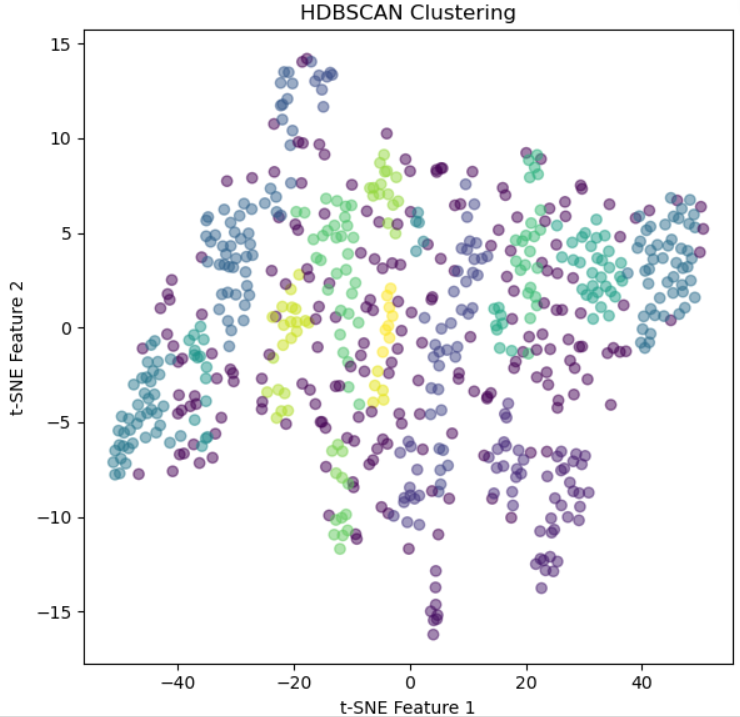
\includegraphics[width=\linewidth]{HDBSCAN.png} 
\caption{HDBSCAN Drug Clustering} 
\label{fig: HDBSCAN clustering} % Label for referencing the image within your text
\end{figure}
 'min\_cluster\_size' in HDBSCAN is used to define the smallest collection of data points in the dataset that HDBSCAN will consider a cluster. This parameter plays a significant role in the resulting cluster structure and is critical for fine-tuning the clustering outcome to suit specific data characteristics and analytical needs. Below image shows the min\_cluster\_size that we achieved by calculating silhouette score. This value can be experimented with, till the results converge. 
\begin{figure}[htbp]
\centering
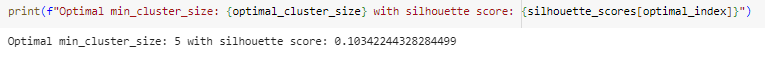
\includegraphics[width=\linewidth]{min_cluster_size_HDBSCAN.PNG} 
\caption{HDBSCAN Drug Clustering - Parameter 'min\_cluster\_size'} 
\label{fig: HDBSCAN clustering} % Label for referencing the image within your text
\end{figure}

Similarly for classifying the DDI as ADR or not, a Node2Vec feature set is created and both the the node feature vectors for both the drugs are appended to create a new feature matrix which corresponds to the entire drug-drug interaction, This dataset, when split into train and test, applying SMOTE and standardscaler,
is experimented as input features for various classifiers like Logistic regression, SGD, and GNN architectures.  

\subsubsection{Logistic Regression}

Logistic Regression is a simple yet effective binary classification algorithm. It is chosen for its compatibility with Node2Vec feature vectors because it provides several advantages:
\begin{itemize}
    \item Interpretability: Logistic Regression produces interpretable results, making it easier to understand the contributions of individual features (Node2Vec embeddings) to the classification decision. This can be crucial in the medical domain, where interpretability and transparency are often essential.
    \item Efficiency: Logistic Regression is computationally efficient and can handle large feature spaces. Node2Vec often generates high-dimensional feature vectors, and Logistic Regression can efficiently process such data.
    \item Efficiency: Logistic Regression is computationally efficient and can handle large feature spaces. Node2Vec often generates high-dimensional feature vectors, and Logistic Regression can efficiently process such data.
    \item Linearity: While Logistic Regression is a linear classifier, it can still capture complex patterns in data when feature vectors are informative. Node2Vec embeddings are designed to preserve structural information in graphs, allowing Logistic Regression to capture nonlinear relationships when projected into the feature space.
\end{itemize}

\subsubsection{SGD Classifier}
SGD is a popular optimization algorithm used to train various machine learning models, including logistic regression. It is chosen for its compatibility with Node2Vec feature vectors due to the following reasons:
\begin{itemize}
    \item Scalability: SGD is well-suited for large datasets, and it can handle high-dimensional feature vectors efficiently. \item Node2Vec embeddings often result in high-dimensional feature spaces, and SGD can cope with the computational demands associated with training on such data.
    \item Flexibility: SGD allows for fine-grained control over the training process. This means you can adjust learning rates, batch sizes, and regularization terms to optimize the model's performance when working with Node2Vec features.
\end{itemize}

\subsubsection{Graph Neural Networks}
Graph Neural Networks are specifically designed for handling graph-structured data, making them a natural choice for compatibility with Node2Vec feature vectors extracted from graph-based datasets like the chchse-decagon dataset. Here are the reasons why GNNs are suitable:
\begin{itemize}
    \item Graph Representation: GNNs are designed to work directly with graph data, making them well-suited for leveraging Node2Vec embeddings, which are derived from the drug interaction network. GNNs can capture complex relational information present in the graph structure.
    \item Message Passing: GNNs use a message-passing mechanism to aggregate information from neighboring nodes in the graph. Node2Vec embeddings inherently capture the local and global structural information in the graph, which can be effectively utilized by GNNs during message passing.
    \item Non-Linearity: GNNs can capture non-linear relationships within the graph data, allowing them to uncover intricate patterns in drug-drug interactions that may not be readily apparent in the raw feature vectors.
\end{itemize}
Logistic Regression provides simplicity and interpretability, SGD offers scalability and fine-tuning options, while GNNs excel at modeling complex graph structures. The training time, and accuracies for the models are below. Traditional models like Logistic Regression often assume independence between features. In the context of DDIs, this assumption may not hold, as the interactions between drugs can be interconnected. Modern approaches, like Graph Neural Networks, relax this assumption by considering the underlying graph structure. 

Below is a short summary of the accuracy and performance metrics which are achieved on the test data. 
\begin{figure}[htbp]
\centering
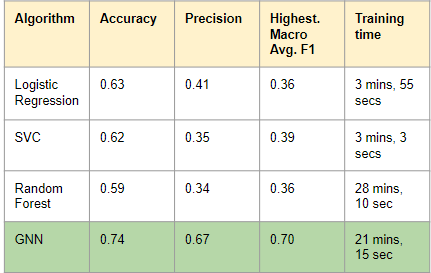
\includegraphics[width=\linewidth]{performance-metrics-1.PNG} 
\caption{Performance of the Models post applying SMOTE to training data} 
\label{fig: Performance Metrics} % Label for referencing the image within your text
\end{figure}

From the above summary, the assumptions about the models have been confirmed, the non-linearity which is compromised in other models, is compensated through GNN, though it takes a longer running time, its a good trade-off where recall, and accuracies are really important. 

Hyperparameters are usually found out by employing RandomGridSearch or GridSearchCV methods, For logistic regression below figure 28 shows the hyperparmeters for Logistic regression post GridSearchCV method

\begin{figure}[htbp]
\centering
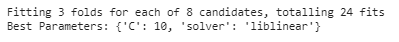
\includegraphics[width=\linewidth]{logistic regression-hyperparameters.PNG} 
\caption{Performance of the Models post applying SMOTE to training data} 
\label{fig: Performance Metrics} % Label for referencing the image within your text
\end{figure}

Logistic Regression, a simple yet effective model, offers two primary hyperparameters that significantly influence its performance. The regularization strength parameter (C) plays a crucial role in balancing overfitting and underfitting. Smaller values of C increase regularization, preventing overfitting but potentially leading to underfitting, while larger values decrease regularization, increasing the risk of overfitting. The choice of solver is another hyperparameter that affects optimization. Different solvers have varying convergence speeds and can impact training time. Careful tuning of these hyperparameters is essential to achieve optimal model performance.

Stochastic Gradient Descent (SGD) is a versatile optimization algorithm used for training various machine learning models. Its hyperparameters include the learning rate (alpha) and the batch size. The learning rate determines the step size taken during each optimization iteration. A higher learning rate may lead to faster convergence but risks overshooting the minimum, while a smaller learning rate can result in slower convergence but increased stability. The batch size determines the number of data points processed in each iteration and impacts memory usage and training speed. Tuning these hyperparameters is critical to finding the right trade-off between convergence speed and stability.

Graph Neural Networks (GNNs) are specialized models for graph-based data, such as drug interaction networks. They offer a range of hyperparameters, including the number of layers, hidden units per layer, learning rate, and dropout. The number of layers and hidden units influence the model's capacity and complexity. Increasing these values can capture more intricate patterns but may also lead to overfitting. Learning rate, similar to SGD, affects the optimization process's convergence speed and stability. Dropout is a regularization technique used to mitigate overfitting by randomly dropping a fraction of neurons' outputs during training. Fine-tuning these hyperparameters in GNNs is crucial to strike the right balance between model complexity, generalization, and training stability.

\section{Evaluation}
For K-means and HDBSCAN, below is the drugs distribution across the clusters. For K-means, the number of clusters were 3, and for HDBSCAN its 5, showing their class distribution here below.

\begin{figure}[htbp]
\centering
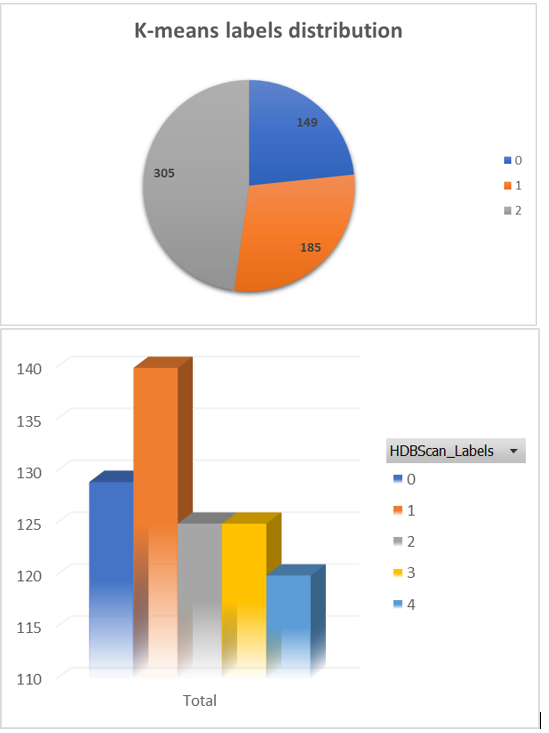
\includegraphics[width=\linewidth]{cluster_results.PNG} 
\caption{Distributions of the Drugs across derived cluster labels} 
\label{fig: Performance Metrics} % Label for referencing the image within your text
\end{figure}

Post Hyperparameter tuning, below are the hyperparameters and their respective values shown in the figure 30

\begin{figure}[htbp]
\centering
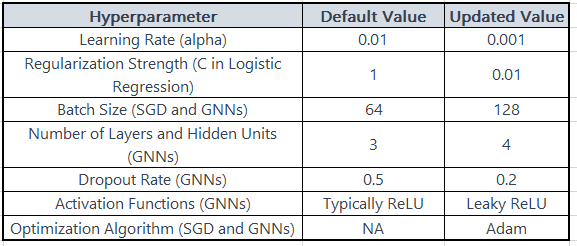
\includegraphics[width=\linewidth]{hyperparmeters tuning.PNG} 
\caption{Hyperparameters and their change} 
\label{fig: Performance Metrics} % Label for referencing the image within your text
\end{figure}

Post Hyperparameter tuning, the accuracies and performance metrics of these models are shown in the below table, 

\begin{figure}[htbp]
\centering
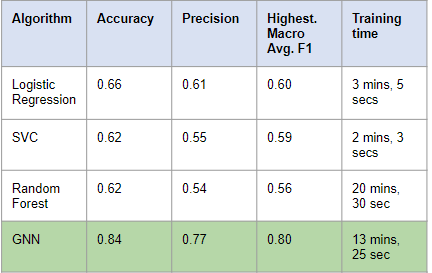
\includegraphics[width=\linewidth]{post_hyper_parameter_tuning.PNG} 
\caption{Post Hyperparmeter tuning testing accuracy with split Node2Vec feature set} 
\label{fig: post-hyper-parameter-tuning} % Label for referencing the image within your text
\end{figure}

The observed improvements in the performance metrics post-hyperparameter tuning indicate a more efficient and effective learning process. For logistic regression, the adjustments in regularization strength and type likely prevented overfitting, resulting in better generalization. For SVC, optimizing the error term penalty and the kernel parameters would have refined the decision boundary to better separate the classes. In the random forest, the increase in the number of estimators and the tuning of tree-specific parameters likely led to a more robust ensemble. Finally, for GNN, the enhancements are attributable to the tuning of the network architecture and learning process, enabling it to better capture and utilize the complex structural information within the graph data, as facilitated by the Node2Vec algorithm.

Below are the class level accuracies for hypertuned, and balanced Logistic Regression, and GNN Models, these metrics on class level signify that the predictions are being accurate for most of the part, Continuous hyperparameter tuning was tried out with Logistic regression, but the model did not converge at all, so the team moved on to GNN. 

\begin{figure}[htbp]
\centering
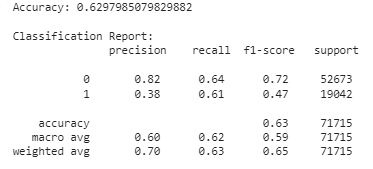
\includegraphics[width=\linewidth]{logistic_regression_post-hyperparmeter.PNG} 
\caption{Class wise Prediction Scores post hyper-parameter tuning for Logistic Regression} 
\label{fig: post-hyper-parameter-tuning} % Label for referencing the image within your text
\end{figure}

Below figure shows the classification accuracy on class level for hypertuned, and SMOTE balanced GNN architecture, Node2Vec hyperparameters were also tuned, resulting the below performance metrics

\begin{figure}[htbp]
\centering
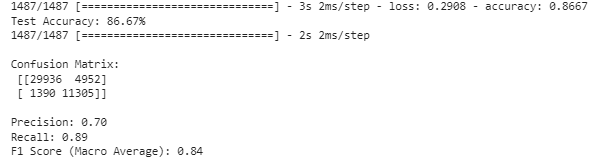
\includegraphics[width=\linewidth]{gnn-post-hyperparameter.PNG} 
\caption{Class wise Prediction Scores post hyper-parameter tuning for GNN} 
\label{fig: post-hyper-parameter-tuning} % Label for referencing the image within your text
\end{figure}

Clearly, the best performing model is GNN which is explained by its compatibility with the Node2Vec extracted features, and the least performing model is Random forest due to its irrelevance to the proposed problem statement. looks like SVM is still affected by the class imbalance which is evident in the class level performance metrics. 

\begin{figure}[htbp]
\centering
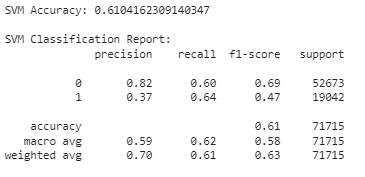
\includegraphics[width=\linewidth]{svm-classlevel.PNG} 
\caption{Class wise Prediction Scores post hyper-parameter tuning for SVM} 
\label{fig: post-hyper-parameter-tuning} % Label for referencing the image within your text
\end{figure}

\begin{figure}[htbp]
\centering
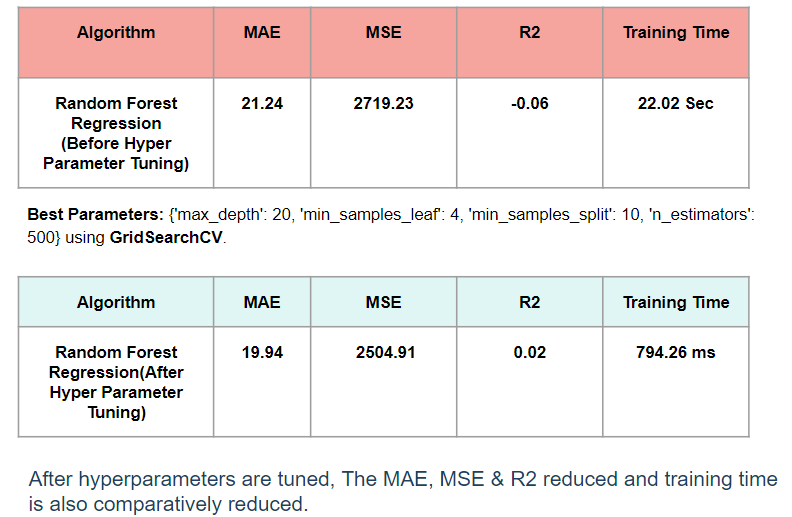
\includegraphics[width=\linewidth]{Model Evaluation 1 Metrics.png} 
\caption{Overall Random Forest Regression Evaluation} 
\label{fig: post-hyper-parameter-tuning} % Label for referencing the image within your text
\end{figure}

\section{Deployment}
The deployment of the project system is designed to handle user scalability and adapt to dynamic environments effectively. The system utilizes Gradio, an open-source Python framework, to deploy machine learning models. Gradio allows for the rapid development of web interfaces that users can interact with, making it suitable for models that require instant feedback and interaction. Gradio's interfaces are hosted on scalable cloud servers that can adjust resources based on user demand. This ensures that the application remains responsive and available, even as the number of users increases. The system is capable of load balancing to distribute user requests efficiently across available resources to maintain performance. Considering the dynamic nature of user environments, Gradio interfaces are designed to be cross-platform compatible, ensuring accessibility across various devices and operating systems. The deployment architecture incorporates containerization, which encapsulates the model and its dependencies in a container. This containerization allows for quick deployment and seamless updates to the system without disruption to the user experience. Gradio facilitates the creation of custom interfaces with input fields tailored to the model's requirements. Users can input data through these fields and receive model outputs in real-time. Interfaces can be embedded into existing websites or accessed via shareable URLs, providing flexibility in how users interact with the models. The system deployment includes security protocols to protect sensitive data and user privacy. Data encryption, secure API endpoints, and user authentication are part of the deployment to ensure safe and secure access. Post-deployment, the system is monitored continuously for uptime, latency, and overall health. Automated alerts are in place for any system anomalies, and a streamlined process for updates and maintenance minimizes system downtime 

\begin{figure}[htbp]
\centering
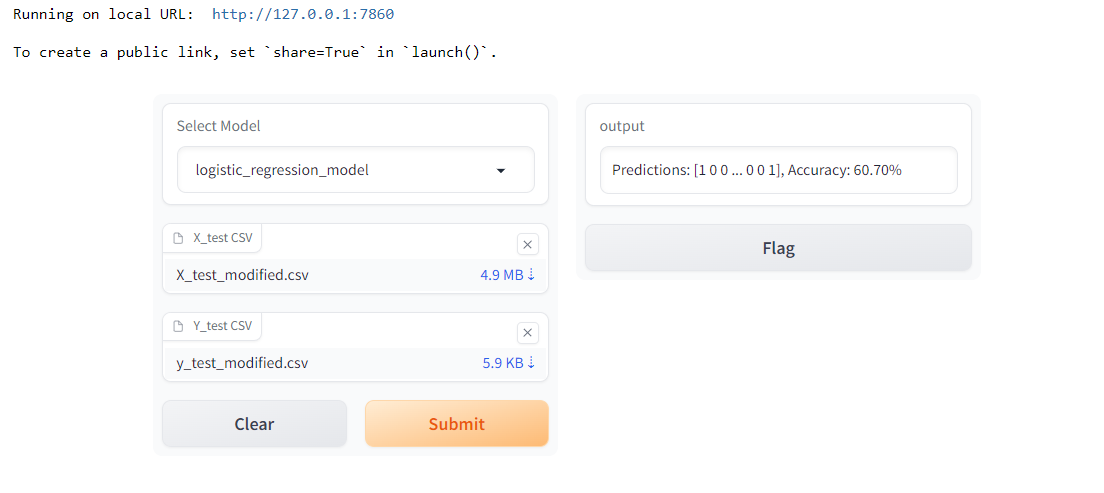
\includegraphics[width=\linewidth]{deployment.png} 
\caption{Deployment of Developed models on Gradio to test the accuracy directly with the test dataset} 
\label{fig: post-hyper-parameter-tuning} % Label for referencing the image within your text
\end{figure}
\section{Conclusion and Future Scope}
In conclusion, the project has achieved its objectives by developing machine learning models that deliver enhanced predictive performance, as substantiated by comprehensive evaluation metrics. The effective application of hyperparameter tuning has resulted in models that not only exhibit high accuracy but also maintain robustness across varied datasets. The deployment via Gradio has allowed for these sophisticated models to be accessible to users through straightforward and interactive web interfaces, bridging the gap between complex machine learning algorithms and practical usability. Looking to the future, the project holds a vast potential for expansion and refinement. There is an opportunity to further refine the models through ongoing optimization techniques and the exploration of cutting-edge algorithms. Deployment strategies can be evolved to incorporate more dynamic cloud services, ensuring scalability and responsiveness to an expanding user base. Enhancing the user experience remains a priority, with iterative interface design improvements driven by user feedback. The inclusion of broader and more diverse datasets will enable the models to learn from a wider array of patterns, potentially increasing their accuracy and generalizability. Introducing real-time analytics could offer users valuable insights into the models' decision-making processes, thereby fostering transparency and trust. With the growth of the user base, maintaining rigorous data security protocols will be paramount to safeguard user privacy.
Furthermore, as edge computing becomes more prevalent, it could be harnessed to decrease latency and augment the efficiency of the deployed models. Finally, and perhaps most importantly, the project will continue to address the ethical considerations of AI, ensuring that the models operate fairly and without bias. The commitment to ethical AI practices will be at the forefront of the project as it evolves, ensuring that it not only leads with innovation but also with integrity and social responsibility.



% needed in second column of first page if using \NaNApubid
%\NaNApubidadjcol



% An example of a floating figure using the graphicx package.
% Note that \label must occur AFTER (or within) \caption.
% For figures, \caption should occur after the \includegraphics.
% 
%
%\begin{figure}[!t]
%\centering
%\includegraphics[width=2.5in]{myfigure}
% where an .eps filename suffix will be assumed under latex, 
% and a .pdf suffix will be assumed for pdflatex; or what has been declared
% via \DeclareGraphicsExtensions.
%\caption{Simulation results for the network.}
%\label{fig_sim}
%\end{figure}

% Note that the NaNA typically puts floats only at the top, even when this
% results in a large percentage of a column being occupied by floats.


% An example of a double column floating figure using two subfigures.
% (The subfig.sty package must be loaded for this to work.)
% The subfigure \label commands are set within each subfloat command,
% and the \label for the overall figure must come after \caption.
% \hfil is used as a separator to get equal spacing.
% Watch out that the combined width of all the subfigures on a 
% line do not exceed the text width or a line break will occur.
%
%\begin{figure*}[!t]
%\centering
%\subfloat[Case I]{\includegraphics[width=2.5in]{box}%
%\label{fig_first_case}}
%\hfil
%\subfloat[Case II]{\includegraphics[width=2.5in]{box}%
%\label{fig_second_case}}
%\caption{Simulation results for the network.}
%\label{fig_sim}
%\end{figure*}
%
% Note that often NaNA papers with subfigures do not employ subfigure
% captions (using the optional argument to \subfloat[]), but instead will
% reference/describe all of them (a), (b), etc., within the main caption.
% Be aware that for subfig.sty to generate the (a), (b), etc., subfigure
% labels, the optional argument to \subfloat must be present. If a
% subcaption is not desired, just leave its contents blank,
% e.g., \subfloat[].


% An example of a floating table. Note that, for NaNA style tables, the
% \caption command should come BEFORE the table and, given that table
% captions serve much like titles, are usually capitalized except for words
% such as a, an, and, as, at, but, by, for, in, nor, of, on, or, the, to
% and up, which are usually not capitalized unless they are the first or
% last word of the caption. Table text will default to \footnotesize as
% the NaNA normally uses this smaller font for tables.
% The \label must come after \caption as always.
%
%\begin{table}[!t]
% increase table row spacing, adjust to taste
%\renewcommand{\arraystretch}{1.3}
% if using array.sty, it might be a good idea to tweak the value of
 %\extrarowheight as needed to properly center the text within the cells
%\caption{An Example of a Table}
%\label{table_example}
%\centering
% Some packages, such as MDW tools, offer better commands for making tables
%% than the plain LaTeX2e tabular which is used here.
%\begin{tabular}{|c||c|}
%\hline
%One & Two\\
%\hline
%Three & Four\\
%\hline
%\end{tabular}
%\end{table}


% Note that the NaNA does not put floats in the very first column
% - or typically anywhere on the first page for that matter. Also,
% in-text middle ("here") positioning is typically not used, but it
% is allowed and encouraged for Computer Society conferences (but
% not Computer Society journals). Most NaNA journals/conferences use
% top floats exclusively. 
% Note that, LaTeX2e, unlike NaNA journals/conferences, places
% footnotes above bottom floats. This can be corrected via the
% \fnbelowfloat command of the stfloats package.





% if have a single appendix:
%\appendix[Proof of the Zonklar Equations]
% or
%\appendix  % for no appendix heading
% do not use \section anymore after \appendix, only \section*
% is possibly needed

% use appendices with more than one appendix
% then use \section to start each appendix
% you must declare a \section before using any
% \subsection or using \label (\appendices by itself
% starts a section numbered zero.)
%


\appendices
\section{GitHub Link}

https://github.com/nikhileasy420/MSDA/tree/main/DATA20245

% Can use something like this to put references on a page
% by themselves when using endfloat and the captionsoff option.
\ifCLASSOPTIONcaptionsoff
  \newpage
\fi



% trigger a \newpage just before the given reference
% number - used to balance the columns on the last page
% adjust value as needed - may need to be readjusted if
% the document is modified later
%\NaNAtriggeratref{8}
% The "triggered" command can be changed if desired:
%\NaNAtriggercmd{\enlargethispage{-5in}}

% references section


%
% <OR> manually copy in the resultant .bbl file
% set second argument of \begin to the number of references
% (used to reserve space for the reference number labels box)
\begin{thebibliography}{1}

\bibitem{howto:kopka}
H.~Kopka and P.~W. Daly, \emph{A Guide to }, 3rd~ed.\hskip 1em plus
  0.5em minus 0.4em\relax Harlow, England: Addison-Wesley, 1999.

\bibitem{han2022}
K. Han et al., “A review of Approaches for Predicting Drug–Drug Interactions Based on Machine Learning,” \emph{Frontiers in Pharmacology}, vol. 12, Jan. 2022, doi: 10.3389/fphar.2021.814858. Available: \url{https://doi.org/10.3389/fphar.2021.814858}.

\bibitem{node2vec}
“Papers with Code - node2vec: Scalable Feature Learning for Networks,” Jul. 03, 2016. Available: \url{https://paperswithcode.com/paper/node2vec-scalable-feature-learning-for}.

\bibitem{bang2021}
S. Bang, J. H. Jhee, and H. Shin, “Polypharmacy side-effect prediction with enhanced interpretability based on graph feature attention network,” \emph{Bioinformatics}, vol. 37, no. 18, pp. 2955–2962, Mar. 2021, doi: 10.1093/bioinformatics/btab174. Available: \url{https://doi.org/10.1093/bioinformatics/btab174}.

\bibitem{zitnik}
M. Žitnik, M. Agrawal, and J. Leskovec, “Modeling polypharmacy side effects with graph convolutional networks,” \emph{Bioinformatics}. Available: \url{https://doi.org/10.1093/bioinformatics/bty294}.

\bibitem{tatonetti2012}
N. P. Tatonetti, P. P. Ye, R. Daneshjou, and R. B. Altman, “Data-Driven prediction of drug effects and interactions,” \emph{Science Translational Medicine}, vol. 4, no. 125, Mar. 2012, doi: 10.1126/scitranslmed.3003377. Available: \url{https://doi.org/10.1126/scitranslmed.3003377}.

\end{thebibliography}



% biography section
% 
% If you have an EPS/PDF photo (graphicx package needed) extra braces are
% needed around the contents of the optional argument to biography to prevent
% the LaTeX parser from getting confused when it sees the complicated
% \includegraphics command within an optional argument. (You could create
% your own custom macro containing the \includegraphics command to make things
% simpler here.)
%\begin{NaNAbiography}[{\includegraphics[width=1in,height=1.25in,clip,keepaspectratio]{mshell}}]{Michael Shell}
% or if you just want to reserve a space for a photo:
% that's all folks
\end{document}


